\documentclass{standalone}
\usepackage{amsmath,amssymb,amsthm}
\usepackage{graphicx}
\usepackage[pdfborder= 0 0 0,citecolor=black,linkcolor=black,colorlinks=true,bookmarksopen=true]{hyperref}
\usepackage[notref]{showkeys}
\usepackage{caption}
\usepackage{subcaption}
\usepackage{xcolor}
\usepackage{algorithm}
\usepackage{algorithmicx}
\usepackage{algpseudocode}
\usepackage{tikz}
\usetikzlibrary{positioning}
\usepackage{tikz-3dplot}
\usepackage{gnuplot-lua-tikz}
\usepackage{pgfplots}
\usepackage{authblk}
\usepackage[pagewise]{lineno}
\usepackage{calc}
\usetikzlibrary{plotmarks}
\author[1,*]{P.A. Browne}
\affil[1]{Department of Meteorology, University of Reading, UK}
\affil[*]{Correspondence to p.browne@reading.ac.uk}
\title{EMPIRE comms version 1 and 2}
\makeatletter \AtBeginDocument{ \hypersetup{pdftitle= {\@title},pdfauthor= {\@author}}} \makeatother

\date{\today}


\begin{document}
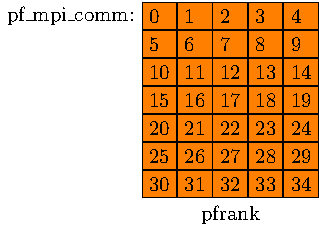
\includegraphics{version_3_pf_mpi_comm}

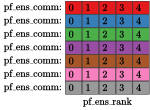
\includegraphics{version_3_pf_ens_comm}

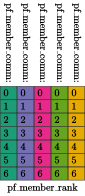
\includegraphics{version_3_pf_member_comm}
\end{document}
